\chapter{Velocità}
\label{sec:velocita}

Le misure ottenute fino ad ora presentano errori derivati dalla precisione non perfetta dell'Object Detection.
Potremmo pensare di  calcolare la velocità $V$ utilizzando l'equazione \ref{eq:vel}
\begin{equation}
    \label{eq:vel}
    \vec{V}_t = \frac{(\vec{P}_t - \vec{P}_{t-1})}{\Delta}
\end{equation}
dove $\vec{P}$ è la posizione reale calcolata in precedenza e $\Delta$ è intervallo tra $t$ e $t-1$.
Calcolare la velocità in questo modo amplifica però gli errori presenti nelle misure di posizione, soprattutto se $\Delta$ è piccolo, e restituisce misure non accettabili.
Possiamo però sfruttare il fatto che $\Delta$ è piccolo per affermare che la differenza tra $\vec{V}_t$ e $\vec{V}_{t-1}$ sia anch'essa piccola.
Possiamo quindi provare a correggere il rumore utilizzando una media mobile esponenziale, come in \ref{eq:ewma}
\begin{equation}
    \label{eq:ewma}
    \vec{V'}_t = k \cdot \vec{V'}_{t-1} + (1-k) \cdot \vec{V}_t
\end{equation}
dove $k \in [0, 1)$ e $V$ è calcolata come in \ref{eq:vel}.
Notiamo però che quest'approccio introduce un ritardo tra i valori calcolati e quelli reali (fig \ref{fig:lag}).
È perciò necessario utilizzare un algoritmo che corregga questo ritardo e allo stesso tempo corregga l'errore in modo simile alla media mobile.

\begin{figure}
    \centering
    \begin{subfigure}[b]{0.45\textwidth}
        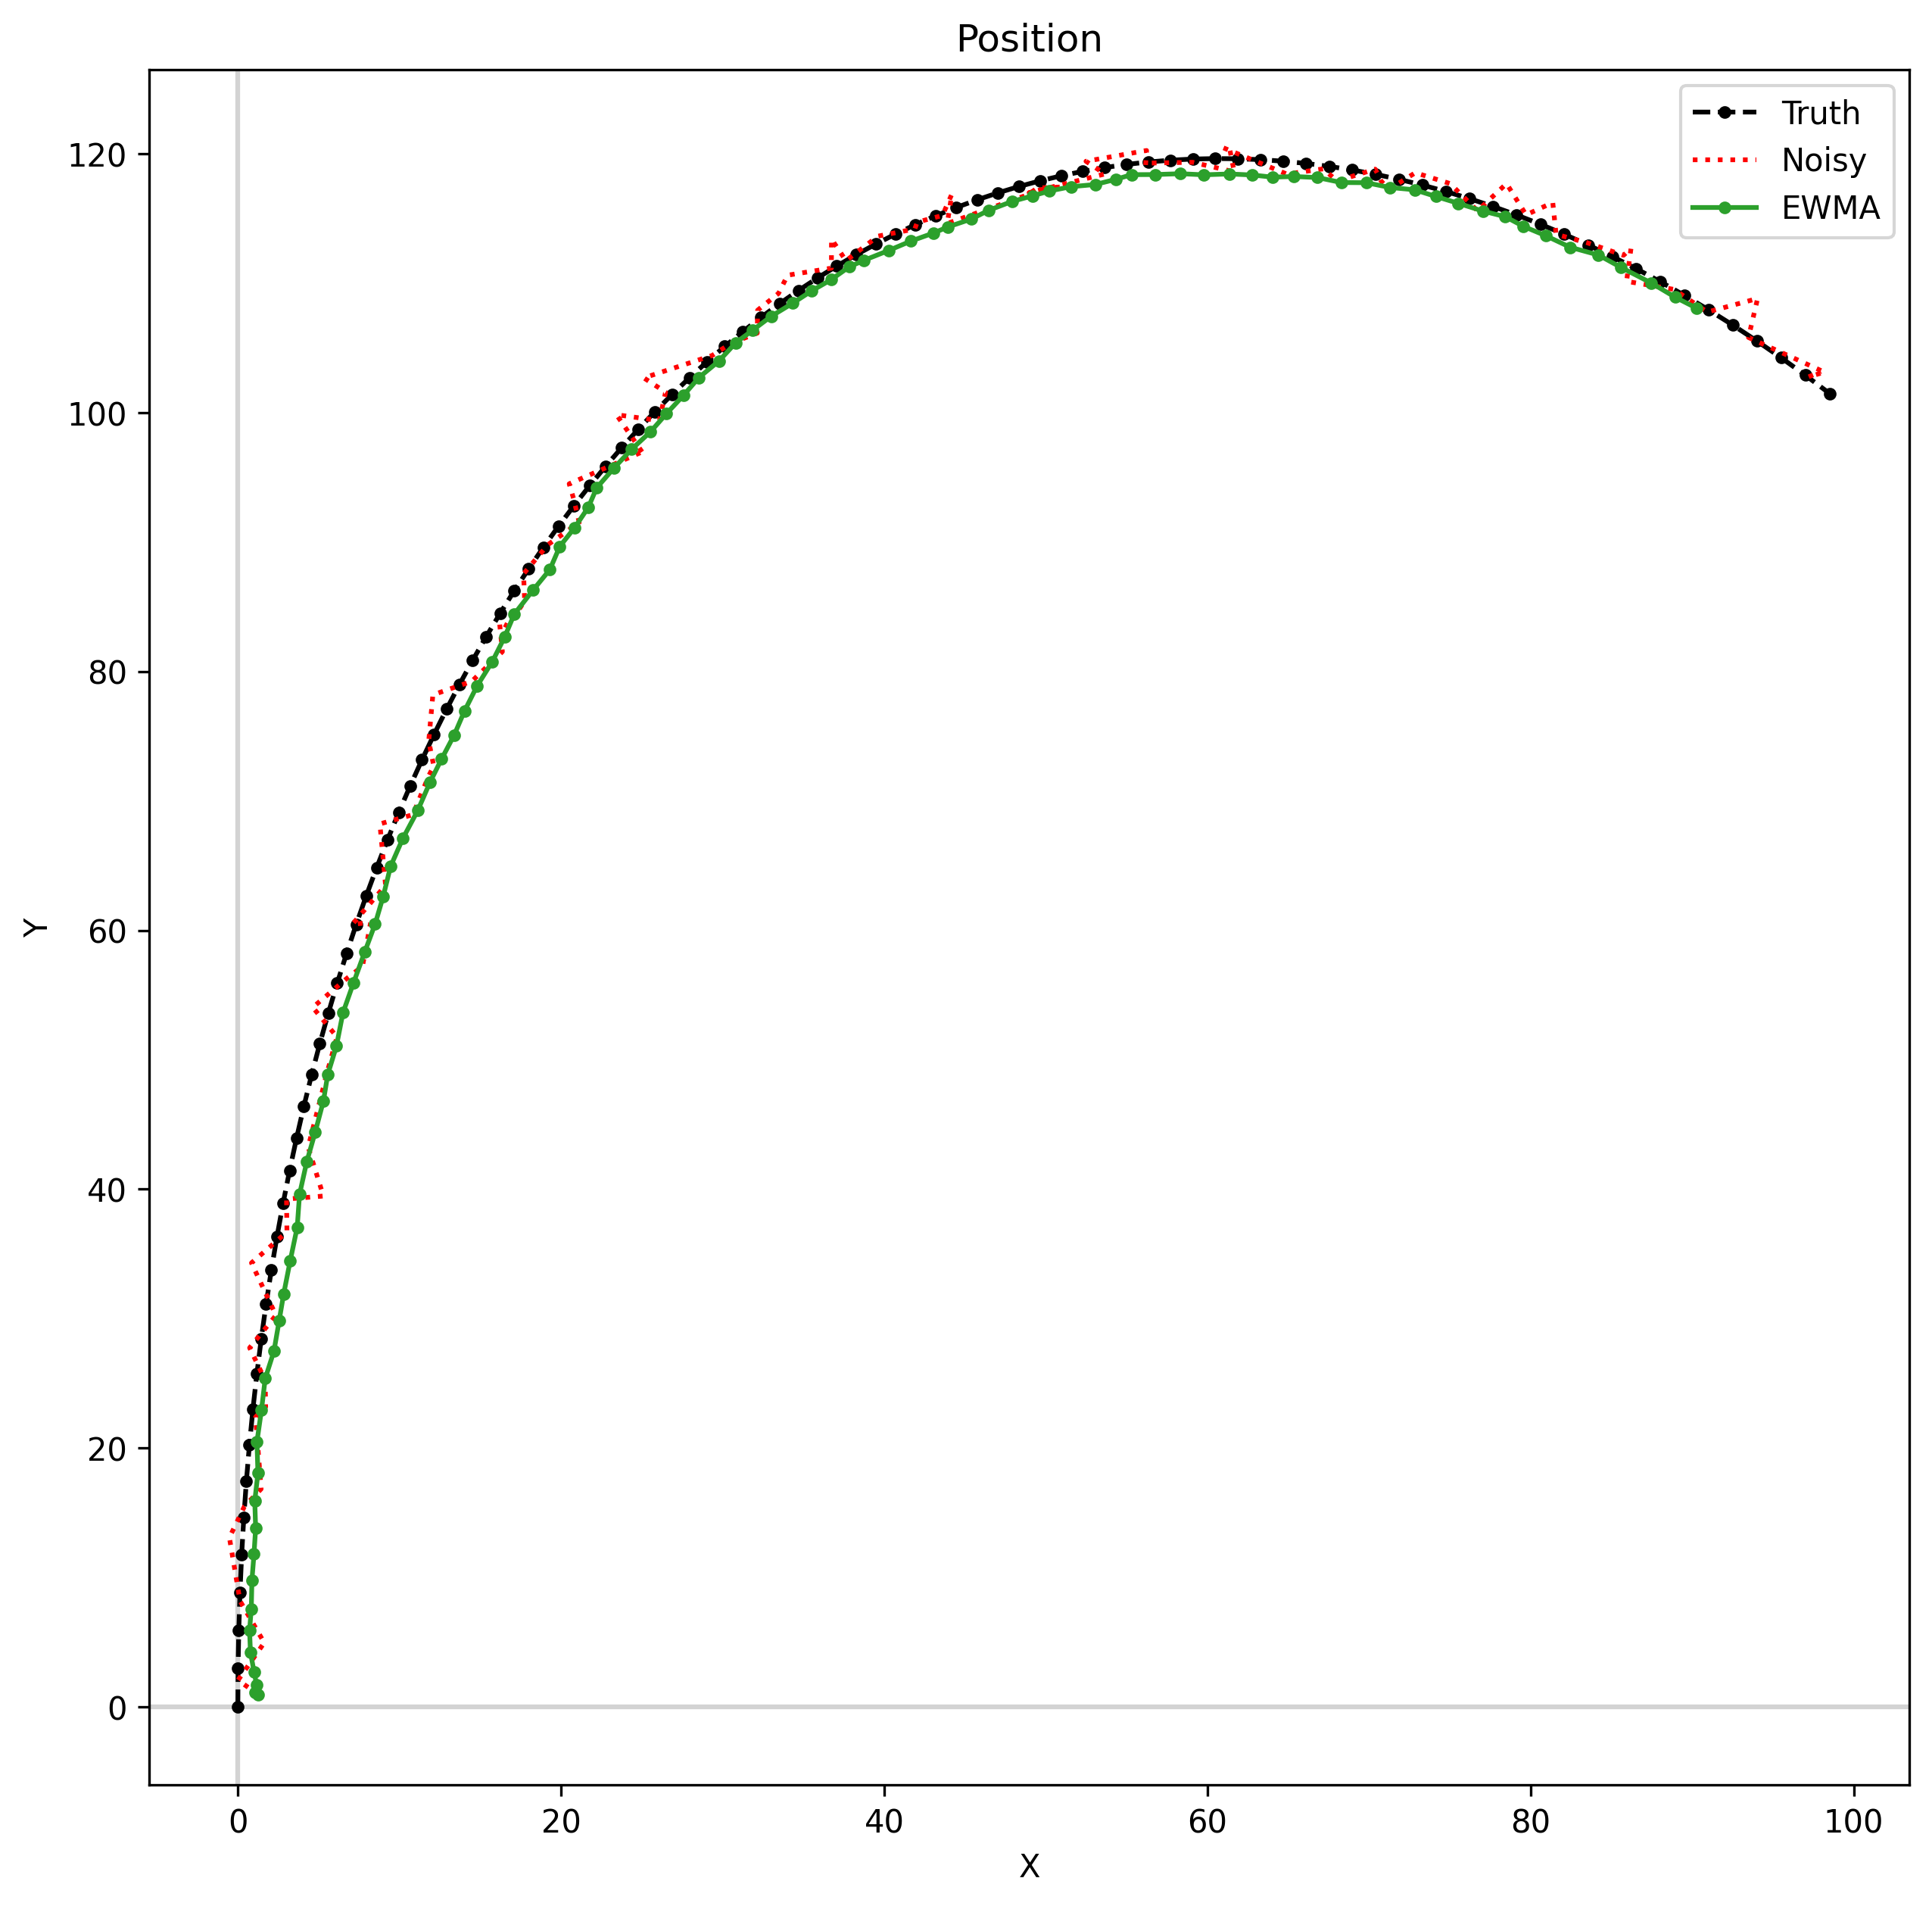
\includegraphics[width=\textwidth]{images/pos0.png}
        \caption{Posizione}
    \end{subfigure}
    \hfill
    \begin{subfigure}[b]{0.45\textwidth}
        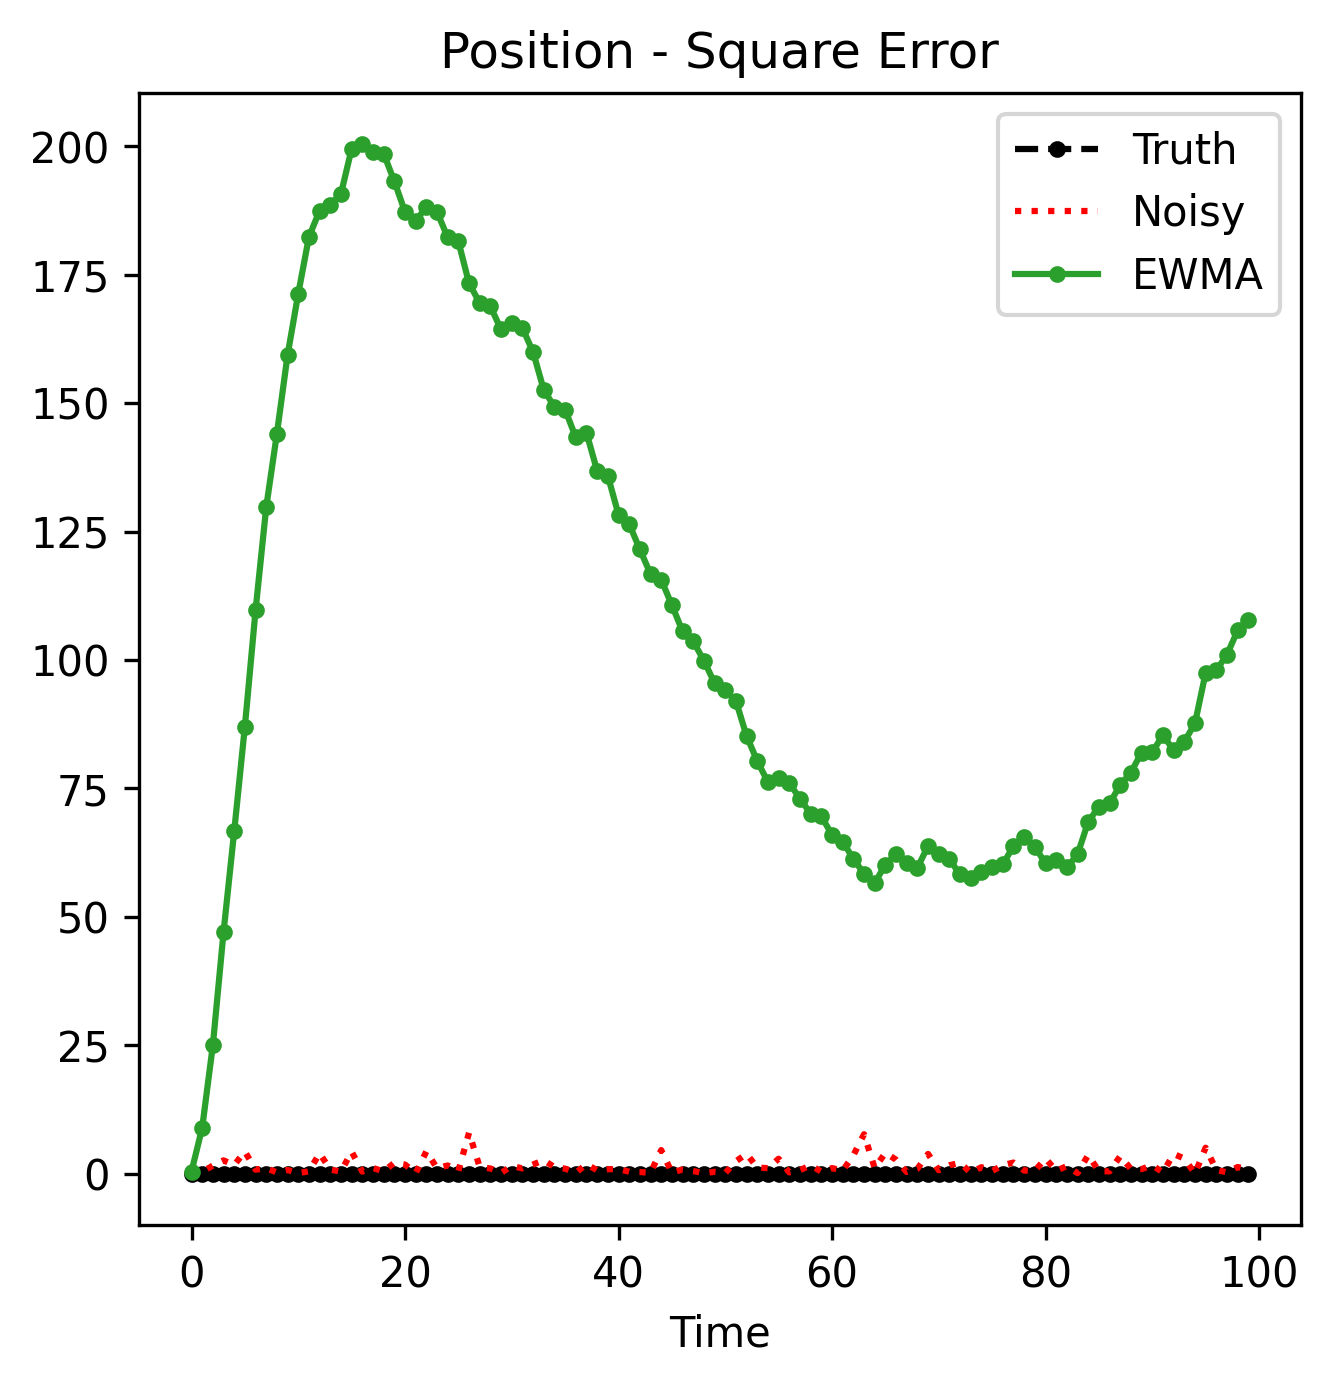
\includegraphics[width=\textwidth]{images/pos0err.png}
        \caption{Errore relativo alla posizione}
    \end{subfigure}
    \vfill
    \begin{subfigure}[b]{0.45\textwidth}
        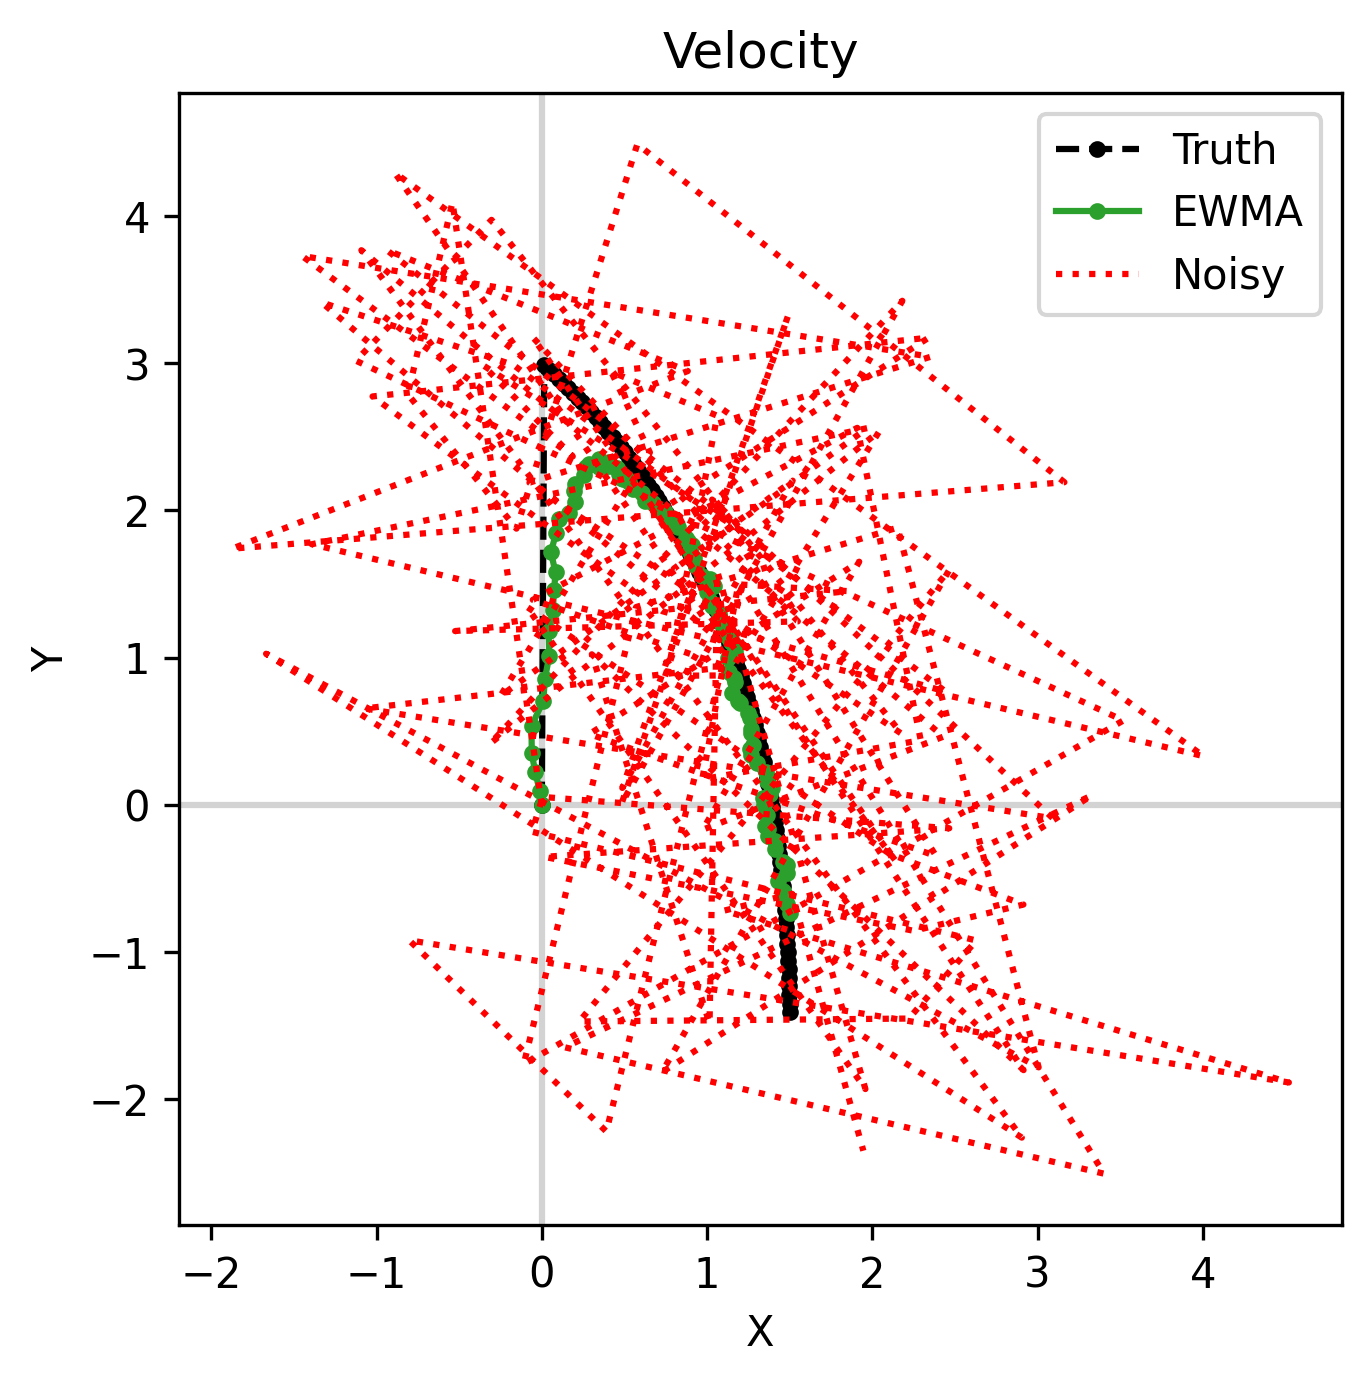
\includegraphics[width=\textwidth]{images/vel0.png}
        \caption{Velocità}
    \end{subfigure}
    \hfill
    \begin{subfigure}[b]{0.45\textwidth}
        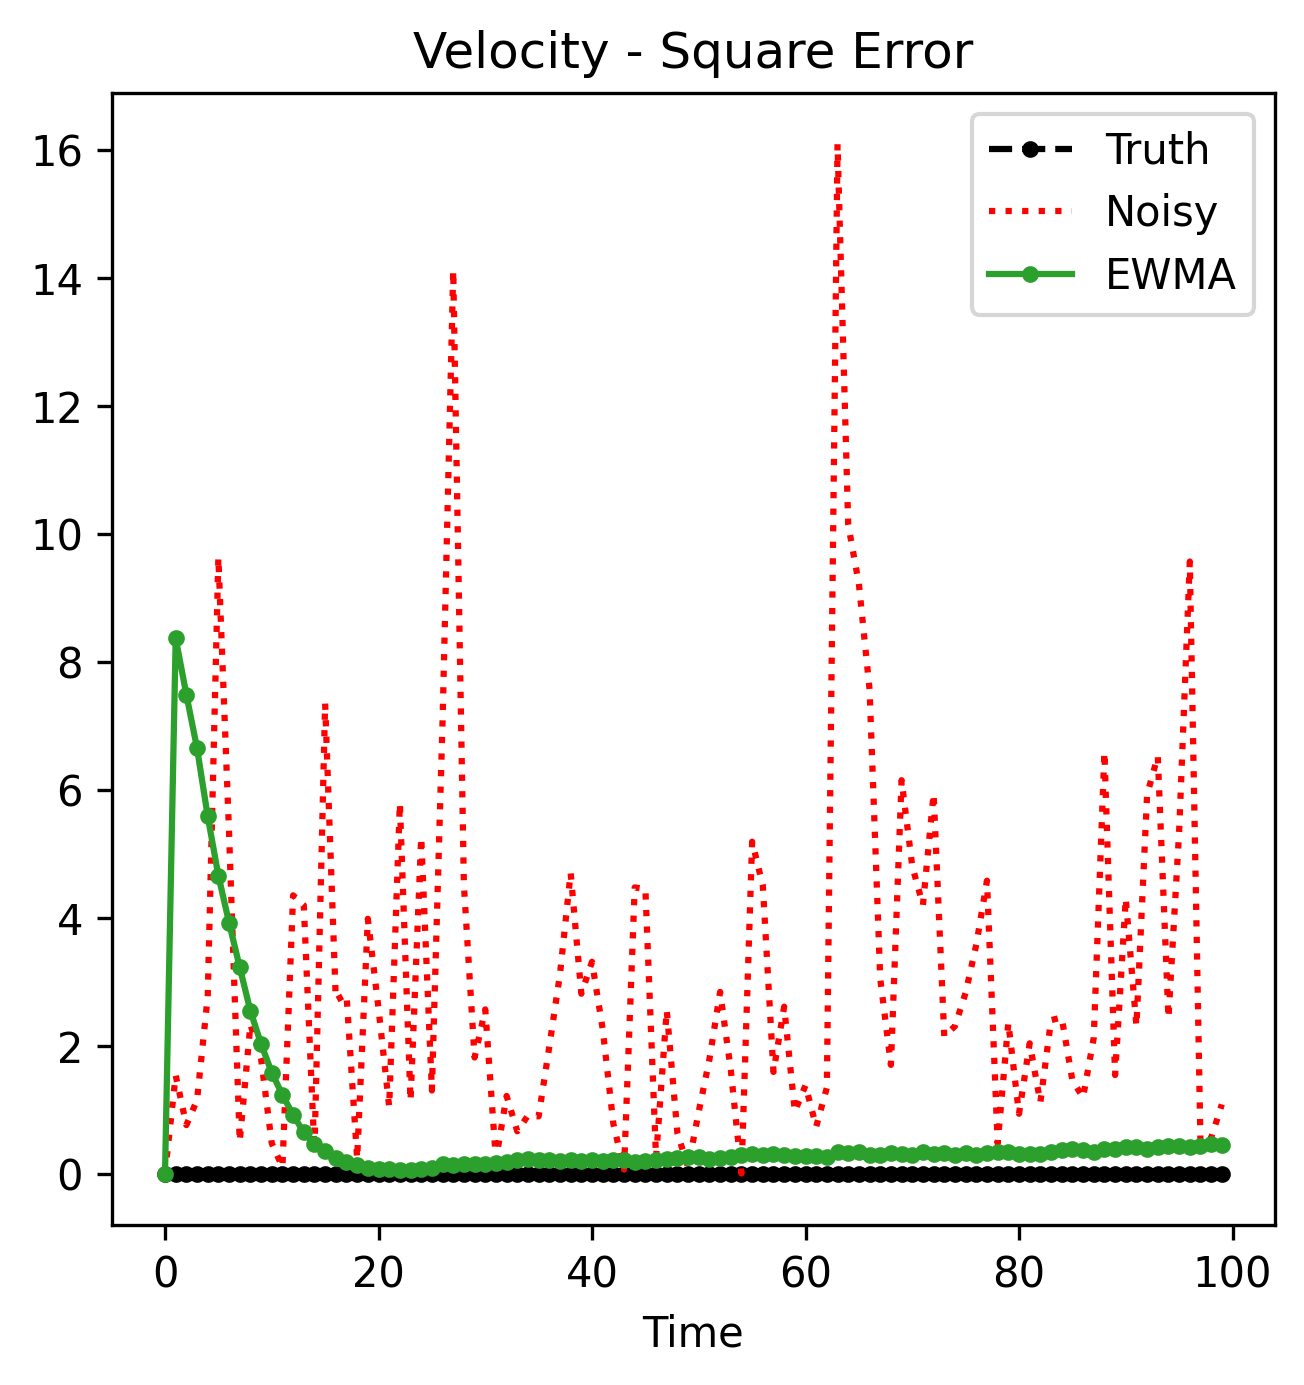
\includegraphics[width=\textwidth]{images/vel0err.png}
        \caption{Errore relativo alla velocità}
    \end{subfigure}
    \caption{Correggere il rumore utilizzando l'EWMA non restituisce risultati accettabili}
    \label{fig:lag}
\end{figure}

L'algoritmo da noi sviluppato è espresso dalle equazioni in \ref{eq:smoothns}
\begin{equation}
    \label{eq:smoothns}
    \begin{split}
        & p'_t = p_{t-1} + v_{t-1} + \frac{1}{2} \cdot a_{t-1} \\
        & v'_t = v_{t-1} + a_{t-1} \\
        & p_t = k \cdot p'_t + (1-k) \cdot P_t \\
        & v_t = k \cdot v'_t + (1-k) \cdot (p_t - p'_t) \\
        & a_t = k \cdot a_{t-1} + (1-k) \cdot (v_t - v'_t) \\
        & \\
        & P'_t = p_t + v_t \cdot \left(\frac{k}{1-k}\right) + \frac{1}{2} \cdot a_t \cdot \left(\frac{k}{1-k}\right)^2 \\
        & V'_t = 2 \cdot \left(v_t + a_t \cdot \left(\frac{k}{1-k}\right)\right)
    \end{split}
\end{equation}
\begin{itemize}
    \item $k \in [0, 1)$ è il coefficiente di correzione
    \item $P_t$ è la posizione osservata all'istante $t$
    \item $p'_t$ è la statistica posizione che ci aspettiamo di avere in base alle nostre conoscenze
    \item $v'_t$ è la statistica velocità che ci aspettiamo di avere in base alle nostre conoscenze
    \item $p_t$ è la statistica relativa alla posizione all'istante $t$
    \item $v_t$ è la statistica relativa alla velocità all'istante $t$
    \item $a_t$ è la statistica relativa all'accelerazione all'istante $t$
    \item $P'_t$ è la posizione corretta all'istante $t$
    \item $V'_t$ è la velocità corretta all'istante $t$
\end{itemize}

Per valutare l'algoritmo sviluppato lo abbiamo messo a confronto con l'algoritmo pubblicato da J.LaViola in \cite{laviola}.
Questo algoritmo è espresso dalle equazioni in \ref{eq:laviola}
\begin{equation}
    \label{eq:laviola}
    \begin{split}
        & Sp_t = \alpha \cdot P_t + (1-\alpha) \cdot Sp_{t-1} \\
        & Sp^{[2]}_t = \alpha \cdot Sp_{t} + (1-\alpha) \cdot Sp^{[2]}_{t-1} \\
        & P'_T = \left(2 + \frac{\alpha \cdot \tau}{1 - \alpha}\right) \cdot Sp_t - \left(1 + \frac{\alpha \cdot \tau}{1 - \alpha}\right) \cdot Sp^{[2]}_t \\
    \end{split}
\end{equation}
\begin{itemize}
    \item $\alpha \in [0, 1)$ è il coefficiente di correzione
    \item $P_t$ è la posizione osservata all'istante $t$
    \item $Sp_t$ è la prima statistica relativa alla posizione all'istante $t$
    \item $Sp^{[2]}_t$ è la seconda statistica relativa alla posizione all'istante $t$
    \item $P'_T$ è la posizione corretta all'istante $T$
    \item $\tau = T - t$ ci permette di predirre la posizione anche in istanti futuri. Nel nostro caso d'uso è sempre uguale a 0.
\end{itemize}
I coefficienti di correzione sono correlati dall'equazione $\alpha = 1-k$.
Il confronto proposto è eseguito con le seguenti condizioni:
\begin{itemize}
    \item $k := 0.85$
    \item $v_0 := a_0 := Sp^{[2]}_0 := [0, 0]$
    \item $p_0 := Sp_0 =: P_0$
    \item Il percorso reale è generato attraverso una curva di Bezier con estremità $[0, 0], [100, 100]$ e punti di controllo $[0, 100], [100, 0]$
    \item Il numero di intervalli è $100$
\end{itemize}
Entrambi gli algoritmi lavorano ad intervalli discreti, e suppongono che le osservazioni siano ad intervalli costanti.
Entrambi correggono la posizione delle entità, e mentre il nostro permette di estrarre in contemporanea informazioni relative alla velocità, per ricavare la velocità dall'altro algoritmo è necessario utilizzare l'equazione \ref{eq:vel} e riapplicare l'algoritmo sui risultati.

\begin{figure}
    \centering
    \begin{subfigure}[b]{0.49\textwidth}
        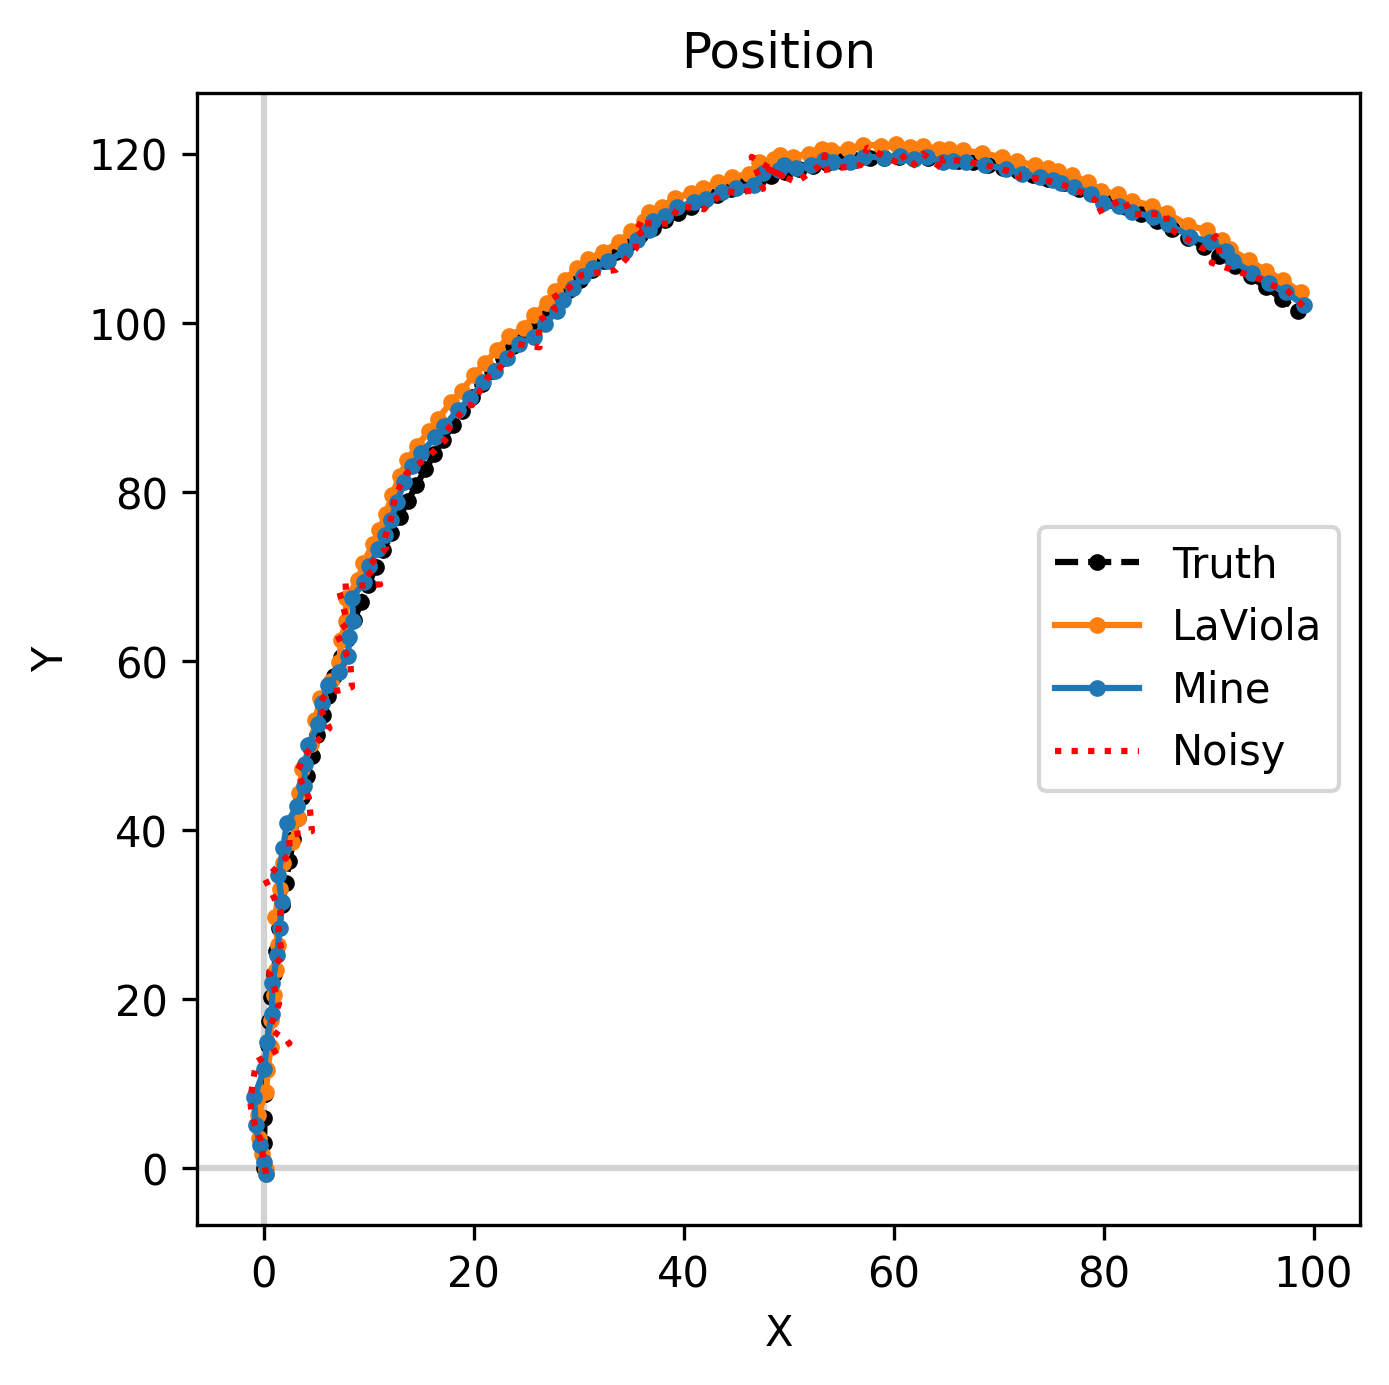
\includegraphics[width=\textwidth]{images/pos1.png}
        \caption{Posizione}
    \end{subfigure}
    \hfill
    \begin{subfigure}[b]{0.49\textwidth}
        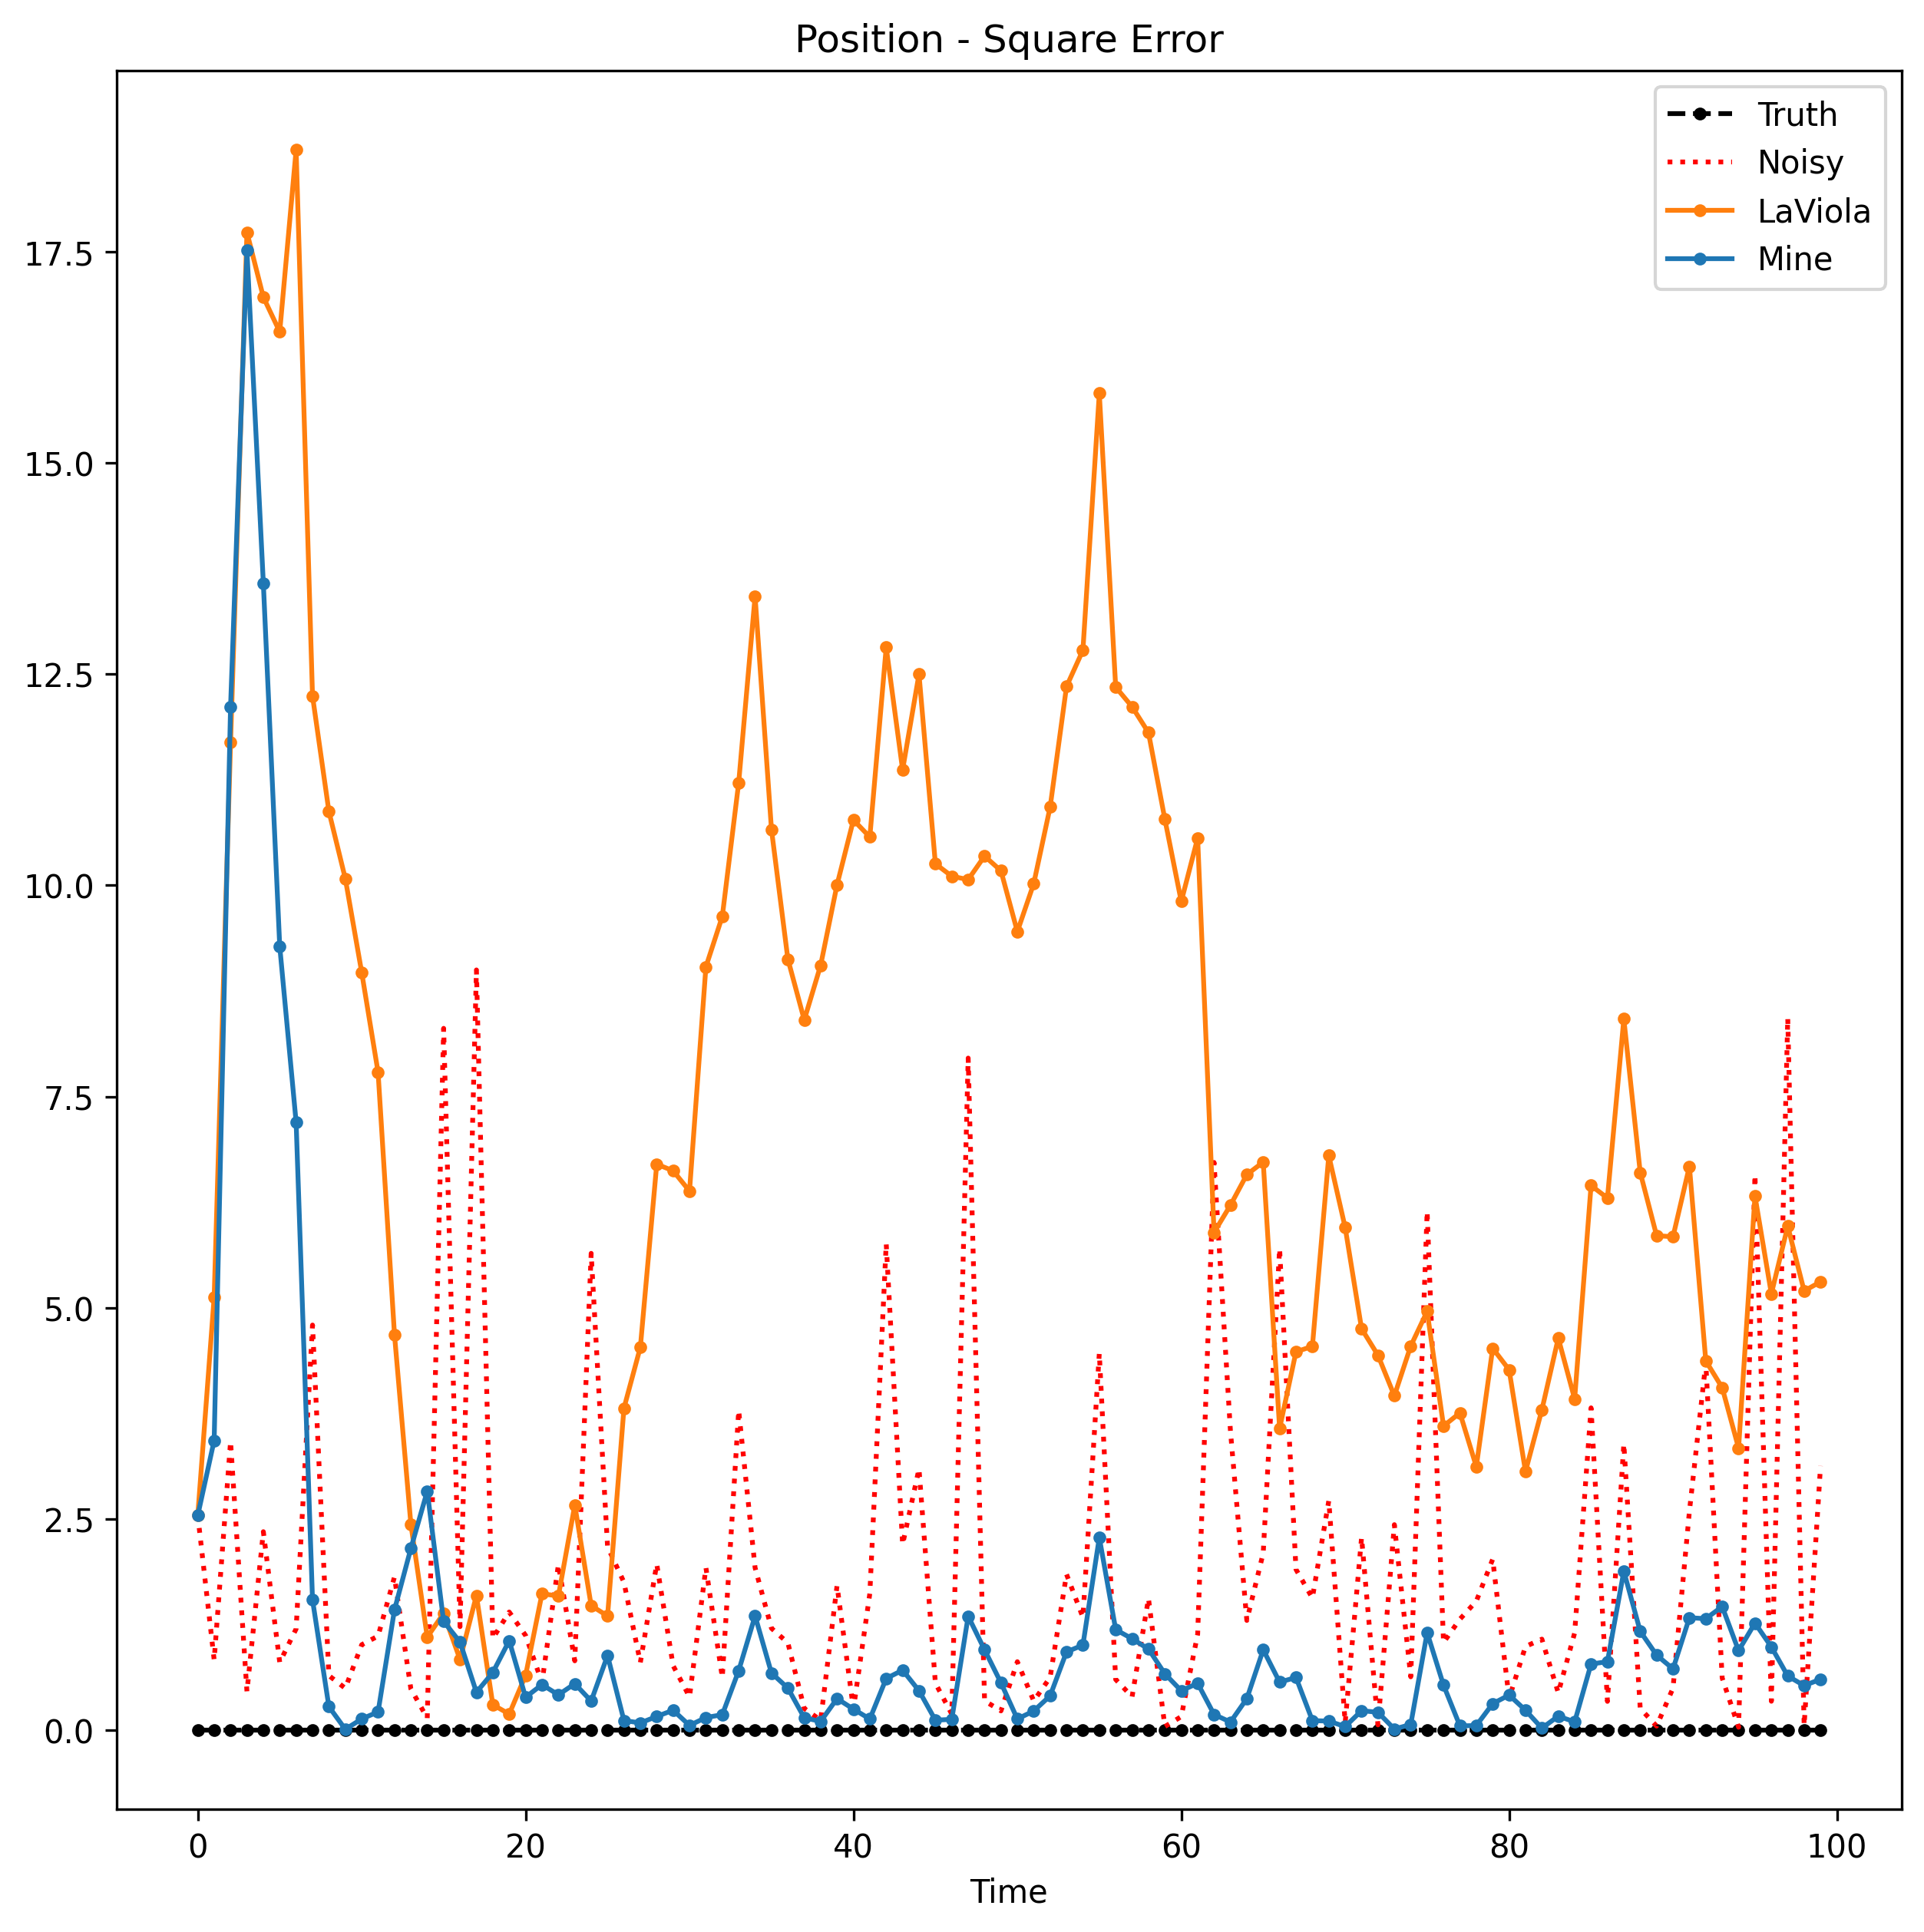
\includegraphics[width=\textwidth]{images/pos1err.png}
        \caption{Errore relativo alla posizione}
    \end{subfigure}
    \caption{Correzione della posizione}
    \label{fig:corrpos}
\end{figure}

\begin{table}
    \caption{Posizione: Errore quadrato medio}
    \label{tab:peqm}
    \centering
    \begin{subtable}{.49\textwidth}
        \caption{da $t=0$}
        \centering
        \begin{tabular}{l r}
            Rumore &    1.9088 \\
            EWMA &    105.9955 \\
            LaViola &   7.2151 \\
            Nostro &    1.2400 \\
        \end{tabular}
    \end{subtable}
    \hfill
    \begin{subtable}{.49\textwidth}
        \caption{ da $t=20$ }
        \label{tab:peqmb}
        \centering
        \begin{tabular}{l r}
            Rumore &   1.8466 \\
            EWMA &   100.4374 \\
            LaViola &  7.1212 \\
            Nostro &   0.5653 \\
        \end{tabular}
    \end{subtable}
\end{table}

\begin{figure}
    \begin{subfigure}[b]{0.49\textwidth}
        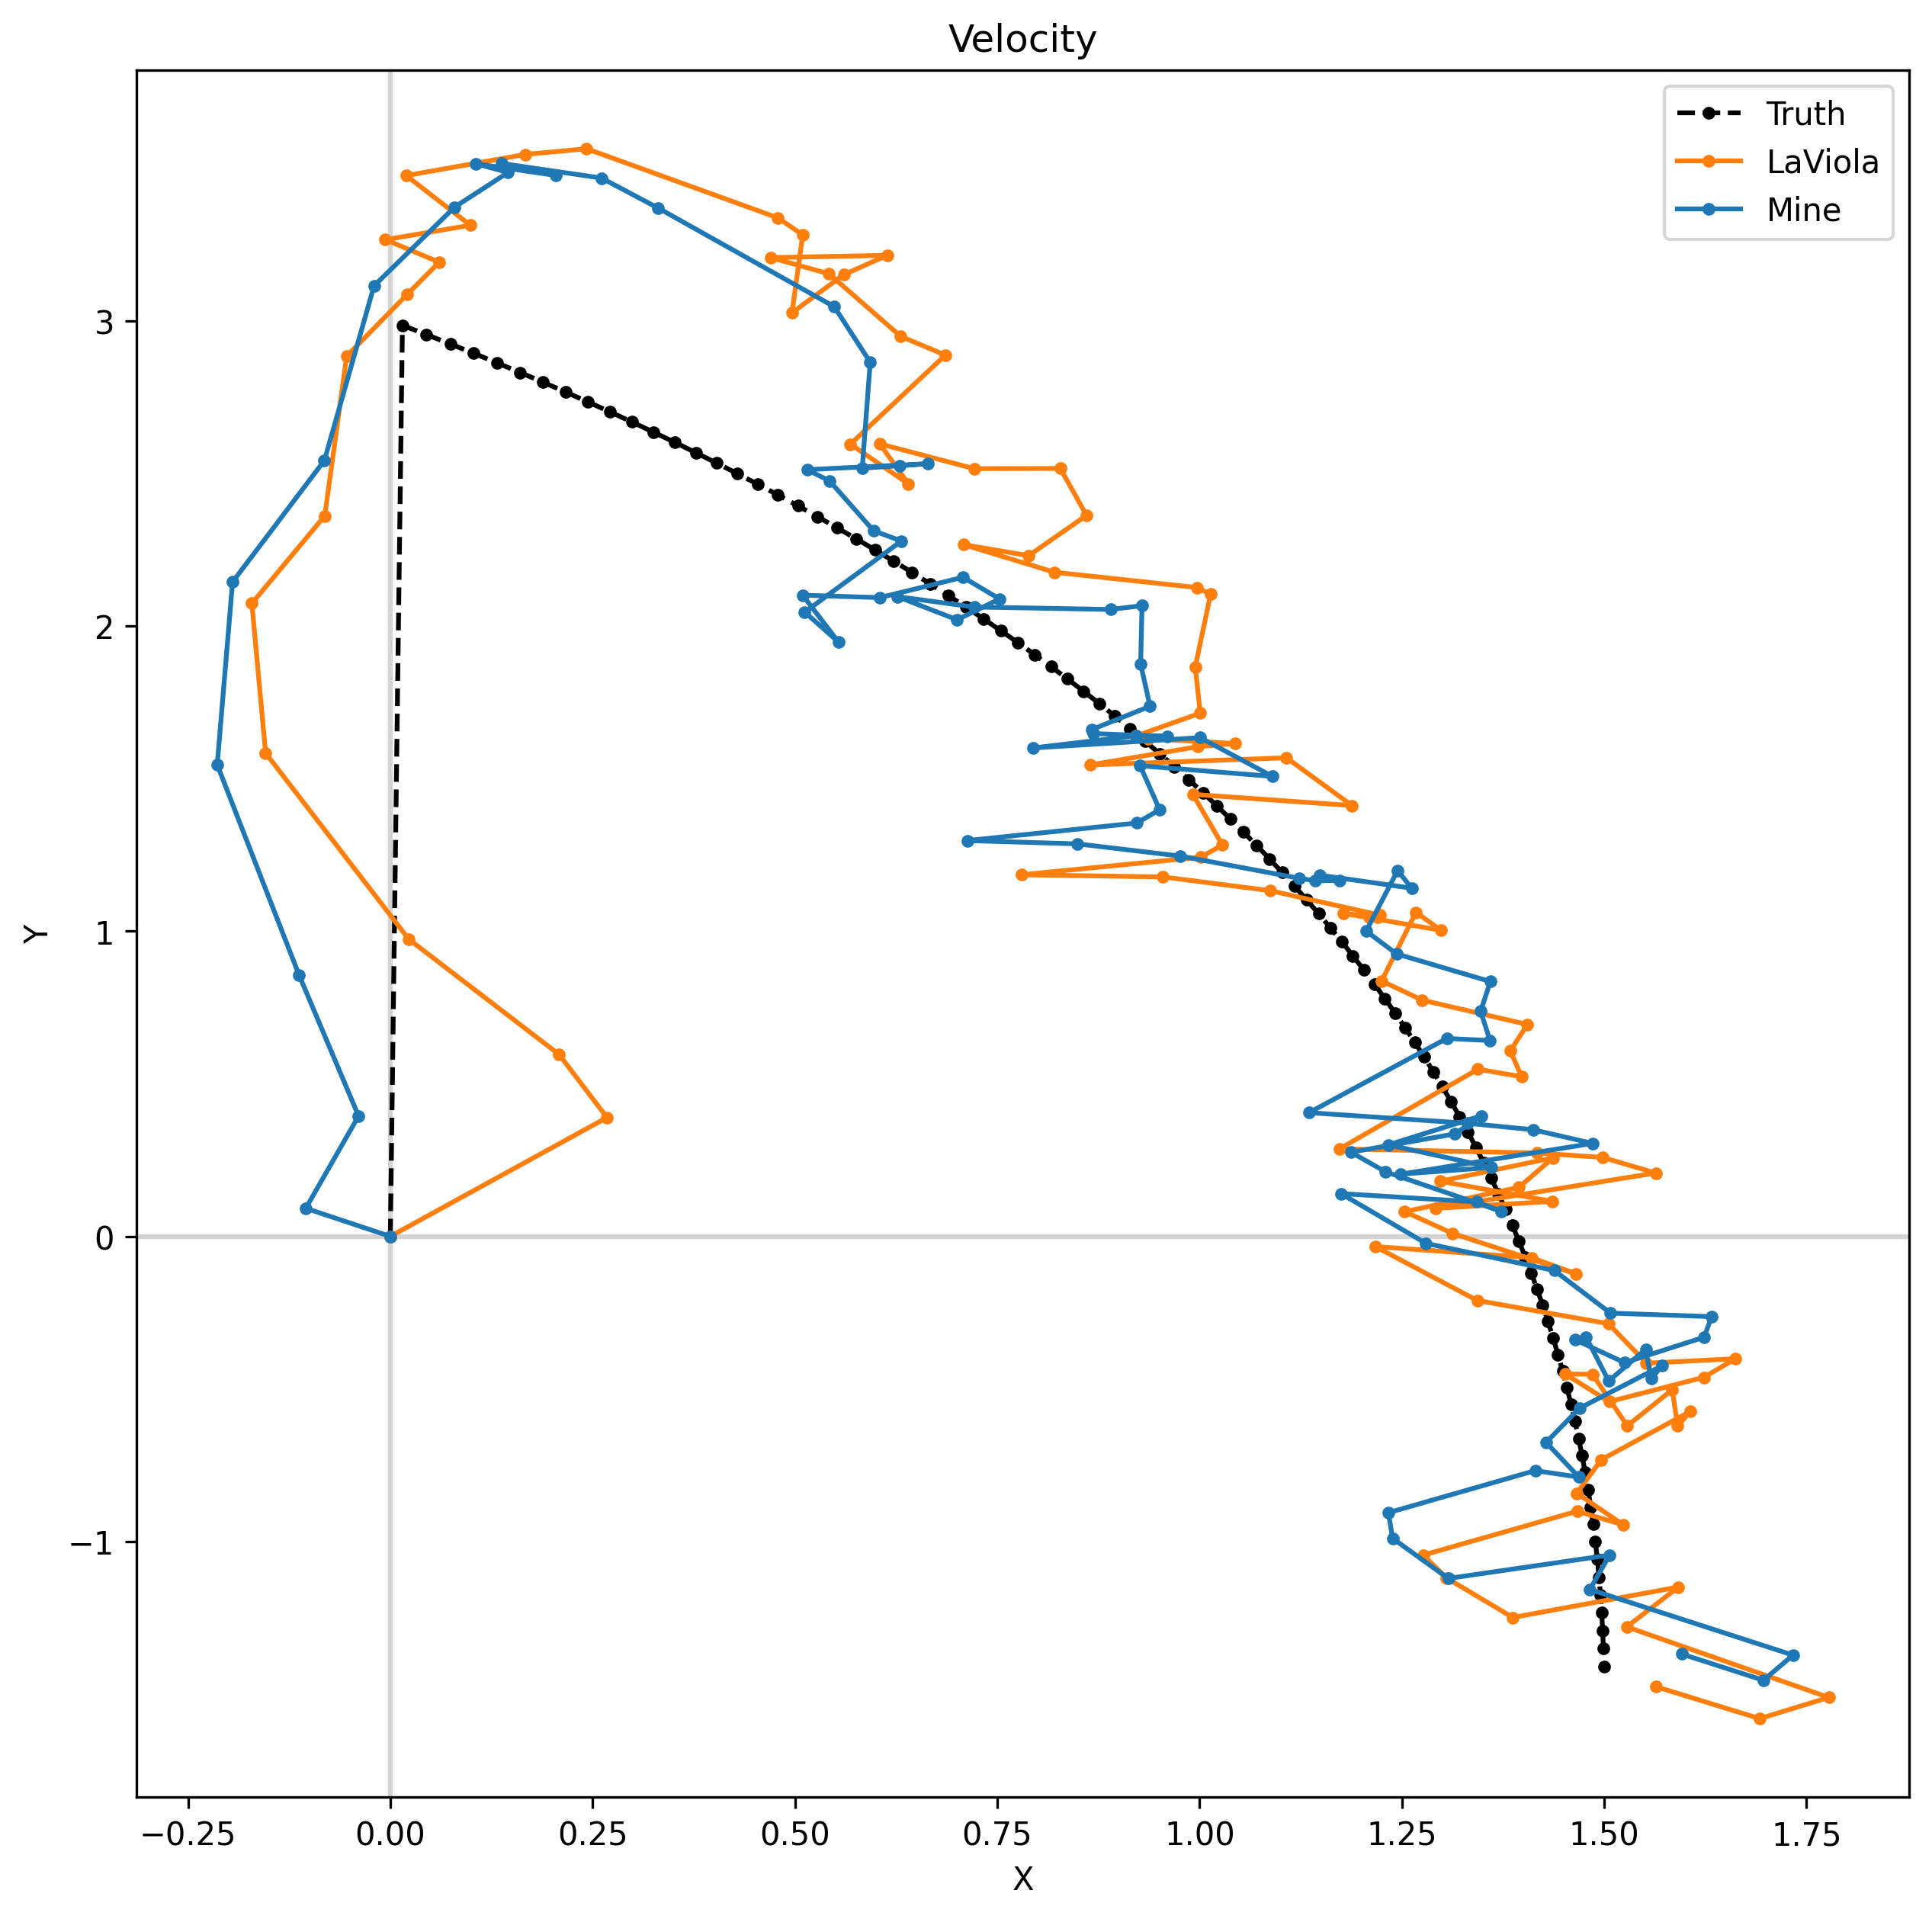
\includegraphics[width=\textwidth]{images/vel1.png}
        \caption{Velocità}
    \end{subfigure}
    \hfill
    \begin{subfigure}[b]{0.49\textwidth}
        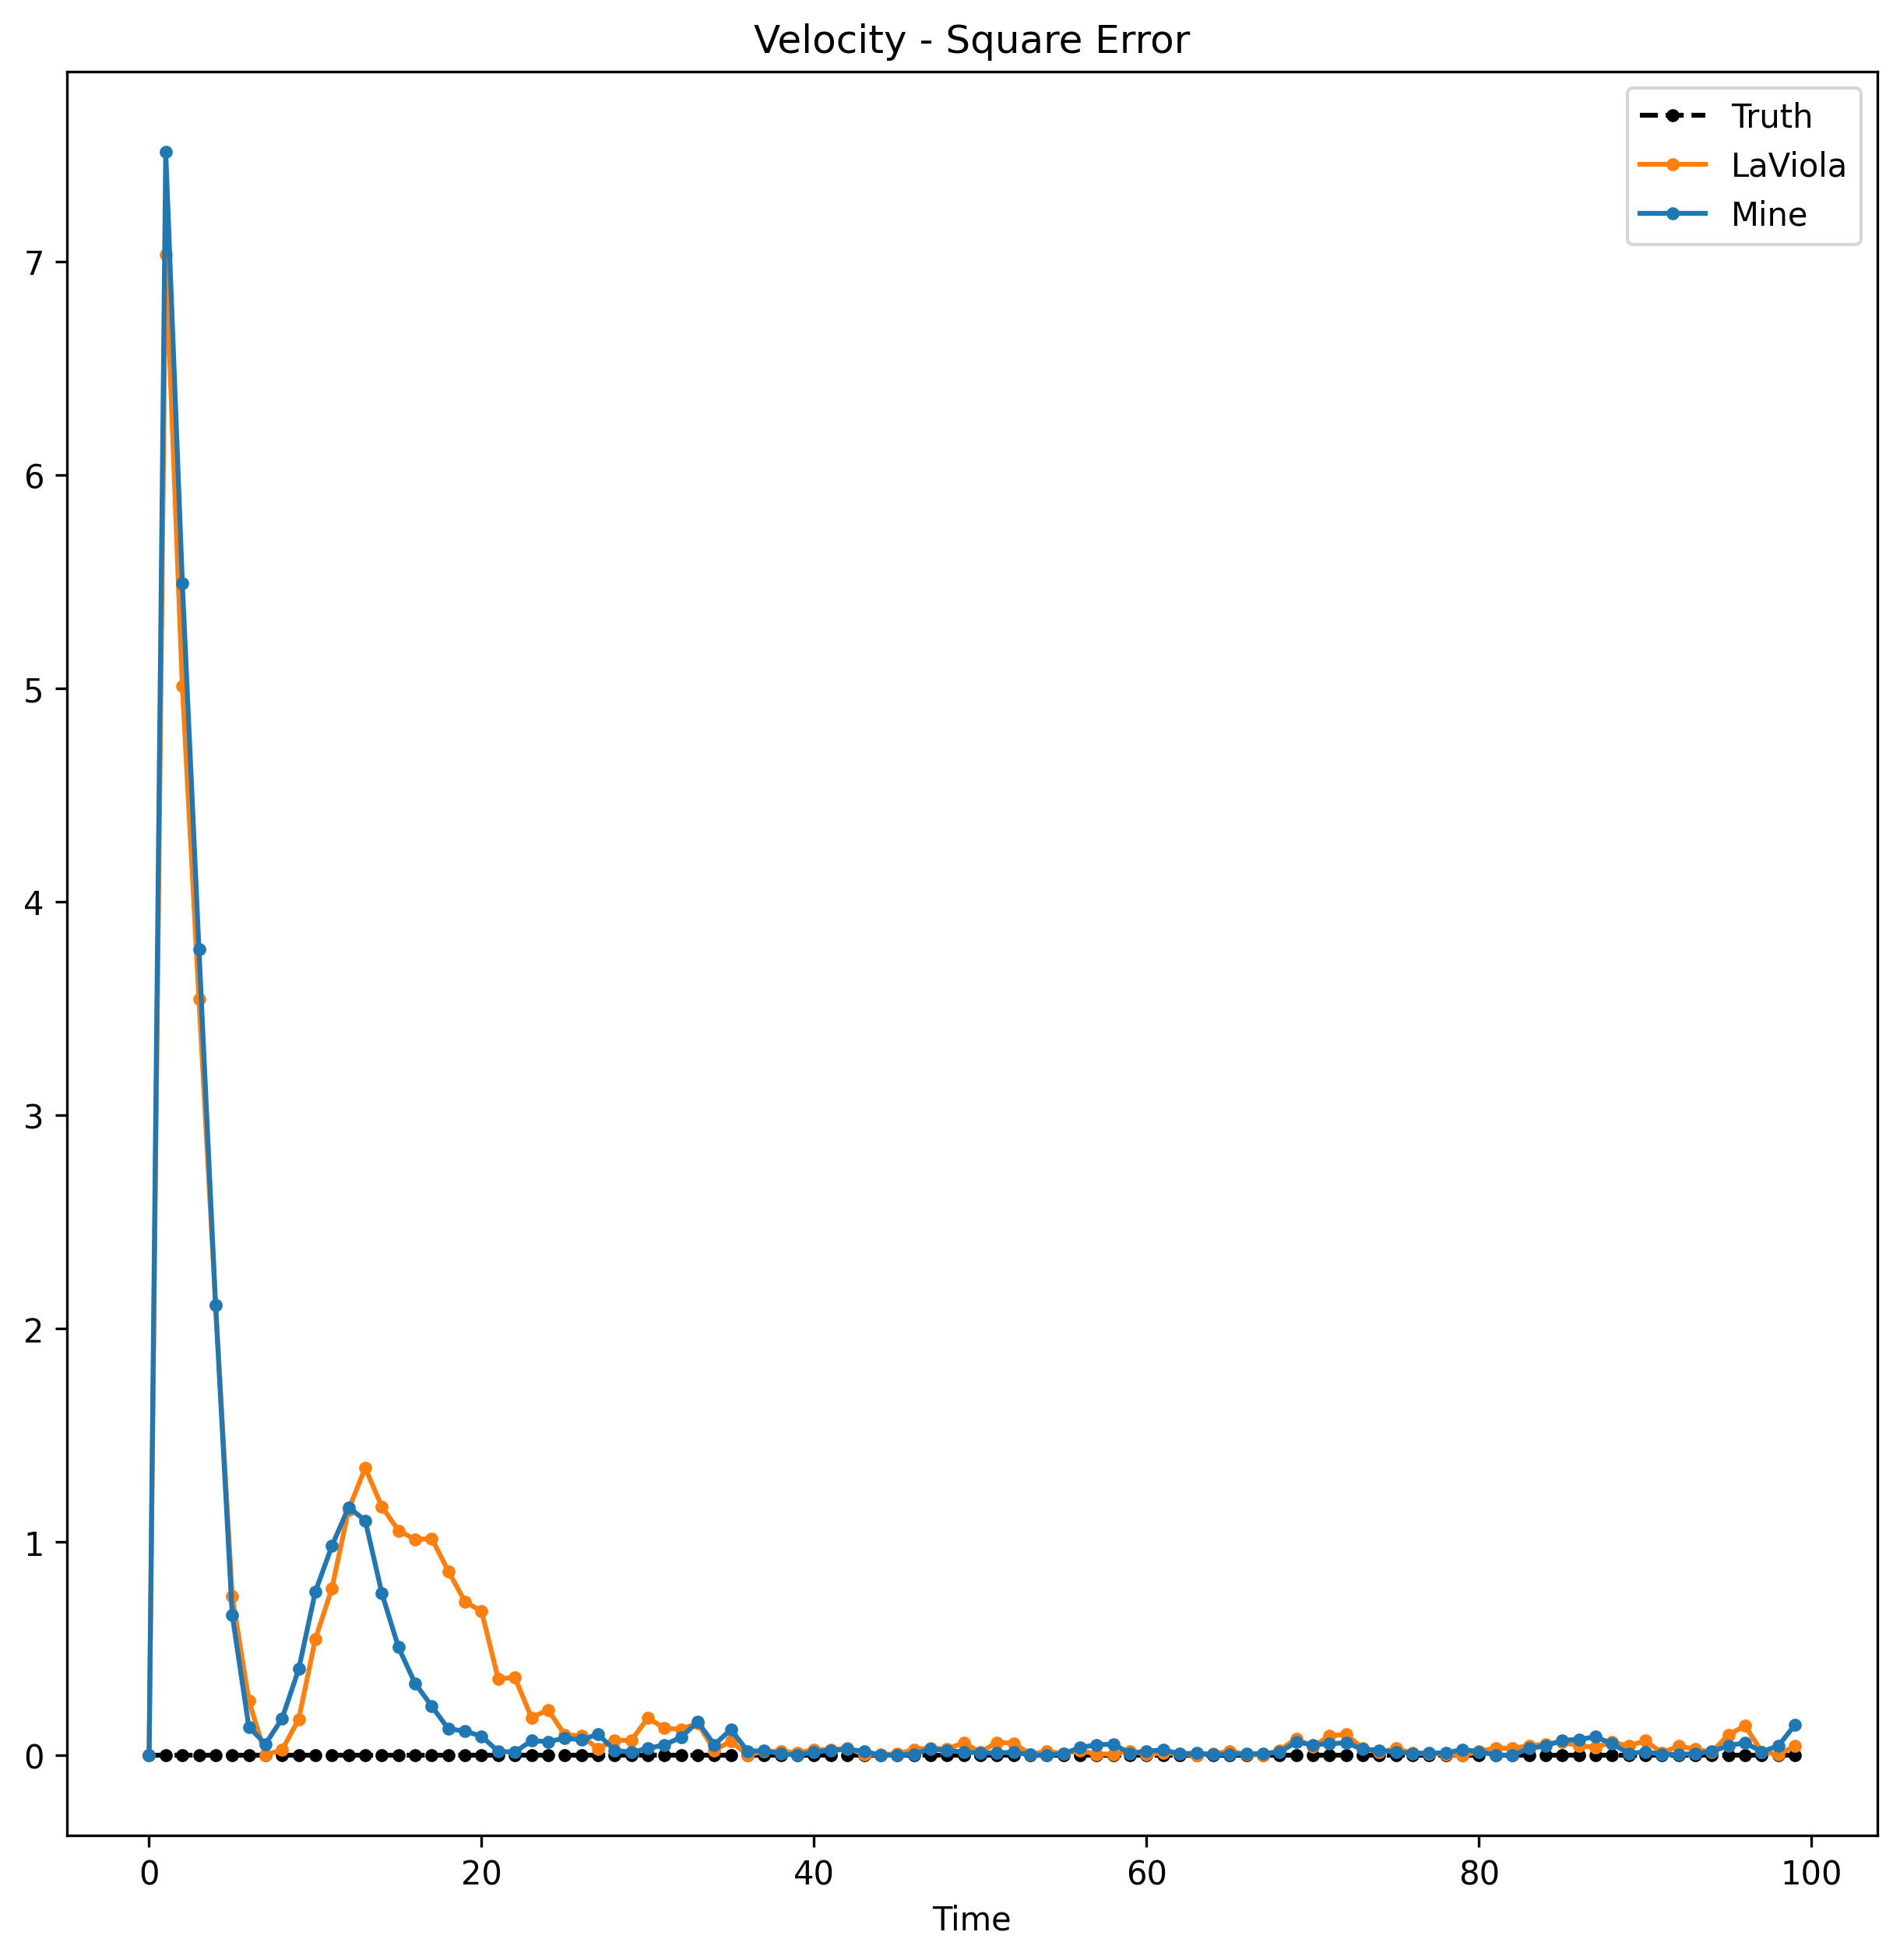
\includegraphics[width=\textwidth]{images/vel1err.png}
        \caption{Errore relativo alla velocità}
    \end{subfigure}
    \caption{Correzione della velocità}
    \label{fig:corrvel}
\end{figure}

\begin{table}
    \caption{Velocità: Errore quadrato medio}
    \label{tab:veqm}
    \centering
    \begin{subtable}{.49\textwidth}
        \caption{da $t=0$}
        \centering
        \begin{tabular}{l r}
            Rumore  & 3.7392 \\
            EWMA    & 0.7734 \\
            LaViola & 0.3136 \\
            Nostro  & 0.2941 \\
        \end{tabular}
    \end{subtable}
    \hfill
    \begin{subtable}{.49\textwidth}
        \caption{ da $t=20$ }
        \label{tab:veqmb}
        \centering
        \begin{tabular}{l r}
            Rumore  & 3.7754 \\
            EWMA    & 0.2837 \\
            LaViola & 0.0694 \\
            Nostro  & 0.0284 \\
        \end{tabular}
    \end{subtable}
\end{table}

L'errore indicato nelle tabelle \ref{tab:peqm} e \ref{tab:veqm} è l'errore quadrato assoluto.
Le alte punte ad inizio esecuzione sono legate all'inizializzazione dei valori dell'algoritmo.
Se inizializzassimo $v$ e $a$ con valori migliori potremmo ridurre gli errori in fase di sincronizzazione e ottenere risultati simili a \ref{tab:peqmb} e \ref{tab:veqmb} sin da inizio esecuzione.
Dai risultati ottenuti si può verificare che il nostro algoritmo ottiene risultati almeno comparabili e apparentemente migliori dell'algoritmo di confronto.
Questo ci da la sicurezza di aver sviluppato un algoritmo corretto e utile, ma valutazioni conclusive sulla sua qualità richiedono test più profondi e confronti con algoritmi diversi.
In particolare sarebbe interessante un confronto con algoritmi basati su Kalman Filter e sue estensioni. 
